\documentclass[12pt]{article}
%\linespread{1.6}

\usepackage{graphicx}
\usepackage{booktabs}
\usepackage{longtable}
\usepackage{tabu}
\usepackage{listings}
\usepackage{hyperref}
\usepackage{tcolorbox}
%\usepackage{neurips_2019}
\usepackage[utf8]{inputenc}
\usepackage[T1]{fontenc}
\usepackage{url}
\usepackage{amsfonts}
\usepackage{nicefrac}
\usepackage{microtype}

\usepackage{amsmath}
\usepackage{amssymb}
\graphicspath{{images/}}
\usepackage{indentfirst}
\usepackage{lipsum}
\usepackage{xcolor}
\usepackage{soul}
\usepackage{setspace}
\usepackage[
backend=biber,
style=alphabetic,
sorting=ynt
]{biblatex}
\usepackage{hyperref}
\usepackage{tikz}
\usetikzlibrary{shapes.geometric, positioning, fit, arrows.meta}

%-----------some colors
\newcommand{\standardcolor}{blue}
\newcommand{\unlimicolor}{red}
\newcommand{\combcolor}{green}

\tikzstyle{startstop} = [rectangle, rounded corners, 
minimum width=3cm, 
minimum height=1cm,
text centered, 
draw=black, 
fill=\standardcolor!30]

\tikzstyle{combFn} = [trapezium, 
trapezium stretches=true, % A later addition
trapezium left angle=70, 
trapezium right angle=110, 
minimum width=3cm, 
minimum height=1cm, text centered, 
draw=black, fill=\combcolor!50,
rounded corners]

\tikzstyle{unlimiFn} = [trapezium, 
trapezium stretches=true, % A later addition
trapezium left angle=70, 
trapezium right angle=110, 
minimum width=3cm, 
minimum height=1cm, text centered, 
draw=black, fill=\unlimicolor!50,
rounded corners]

\tikzstyle{standardFn} = [trapezium, 
trapezium stretches=true, % A later addition
trapezium left angle=70, 
trapezium right angle=110, 
minimum width=3cm, 
minimum height=1cm, text centered, 
draw=black, fill=\standardcolor!50,
rounded corners]

\tikzstyle{process} = [rectangle, 
minimum width=3cm, 
minimum height=1cm, 
text centered, 
text width=3cm, 
draw=black, 
fill=orange!30]
\tikzstyle{decision} = [ellipse, rounded corners,
minimum width=3cm, 
minimum height=1cm, 
text centered, 
draw=black, 
fill=\standardcolor!30]
\tikzstyle{arrow} = [thick,->,>=stealth]
%\usepackage{endfloat}
\addbibresource{sections/references.bib}
\singlespacing
\addtolength{\oddsidemargin}{-.5in}
\addtolength{\evensidemargin}{-.5in}
\addtolength{\textwidth}{1in}

\addtolength{\topmargin}{-.5in}
\addtolength{\textheight}{1in}

\DeclareMathOperator{\softmax}{softmax}
%-----------------------------------------------------------

\begin{document}
%\begin{titlepage}
\begin{center}
\large
\textbf{Project Proposal}\\
\Large
\textbf{Long Document Summarization:}\\
\textbf{Augmenting Unlimiformer with Knowledge Graphs\footnote{\today}}\\
\begin{table}[h]
    \centering
    \begin{tabular}{ccc}
        Patrick O'Callaghan&  Sheel Sansare& Tristan Wang\\
         (patocal)& (ssansa2)  & (aawang99)\\
    \end{tabular}
%    \caption{Caption}
    \label{tab:my_label}
\end{table}
\end{center}
%\end{titlepage}

%\section*{Summary}
Place summary here.
\section{Extracting Knowledge Graphs from Long Documents}
\subsection*{REBEL}
We use REBEL because it is end-to-end (it finds entities and relations simultaneously), open-source, and easy to implement using Hugging Face. Additionally, as per 
the DocRED paper by Yao et al \cite{yao2019DocRED}, pretrained REBEL currently yields the best joint entity and relation extraction (NER and RE) results compared with 
the benchmark among all models sampled, achieving a relation F1 score of 47.1\footnote{https://paperswithcode.com/sota/joint-entity-and-relation-extraction-on-3}.

Since the pre-trained REBEL model has a token limit, we split the LD into 128-token chunks before extracting 3 head-relation-tail triplets from each chunk. We 
split the text into 128 token chunks as it is approximately the length of one paragraph. Through visual inspection, we find that there are typically 3 triples 
in each paragraph. Moreover, since REBEL employs beam search, the number of triples must be less than or equal to the number of beams. We determine that the optimal number 
of beams, based on runtime, is 3 beams, which means the maximum triples per chunk would be 3.

Once the triplets are extracted, we use NetworkX to create a directed graph, and employ MatPlotLib to visualize and plot the results. Below is a sample image of a knowledge 
graph produced from a gold summary.

[Insert Image/Plot of KG]


**Why extract triplets (and not extract triplets typed)?**
\subsection*{DyGIE++} Another relation extraction method we explored for
building KGs is DyGIE++ which refines and scores text spans designed to capture
both intra-sentence and cross-sentence context. We have cloned the code from
the official GitHub repository (\url{https://github.com/dwadden/dygiepp}) and
attempted to replicate the process of training a model for relation extraction
on the SciERC dataset, but have not yet been successful due to technical
difficulties. To resolve this issue, we aim to raise a GitHub issue and
continue to debug as needed, in anticipation that DyGIE++ may be used later on
in our project.

\subsection*{LlamaIndex}
\texttt{LlamaIndex} is a framework for connecting data sources for
Large-Language Models. In particular \texttt{LlamaIndex} has a class called
\texttt{KnowledgeGraphIndex}. We have established that the latter is compatible
with \texttt{FAISS} which is the datastore that \texttt{unlimiformer} uses to
conduct a $k$-nearest neighbor search of top-level hidden state encodings that
are most relevant to the query.
\url{https://github.com/run-llama/llama_index/issues/8767}.
This means that we can store the Knowledge Graph we create using LlamaIndex as
a FAISS datastore. The idea is to create a secondary channel for the attention
mechanism. The potential advantage is characterised in the following notebook:
\href{https://github.com/run-llama/llama_index/blob/main/docs/examples/index_structs/knowledge_graph/KnowledgeGraphIndex_vs_VectorStoreIndex_vs_CustomIndex_combined.ipynb}{KG-datastore-notebook}.
If a nearest neighbor search over a KG produces fewer, but more relevant
results, this may help focus the cross-attention mechanism on what is most
important (see figure \ref{fig-kg-datastore-example}).


\section{Understanding and Implementing Unlimiformer}
\subsection*{Unlimiformer}
**Why unlimiformer, and what is it?**
\section{Next Steps}

One next step would be
fine-tuning the REBEL model on the long-document summarization datasets we
chose, namely the Hugging Face versions of GovReport \cite{huang2021efficient} 
and BookSum \cite{kryscinski2021booksum}. The REBEL model is proven to be
relatively flexible, having been fine-tuned on at least 4 widely-used relation
extraction (RE) datasets of diverse contexts (CONLL04, DocRED, NYT, and ADE)
and performed well on most of them. However, we bear in mind that the 4
aforementioned datasets differ significantly from the one we propose. DocRED
and ADE entities are words or short phrases, while CONLL04 and NYT entities are
sentences from news articles. On the other hand, the entities in our dataset
will be summaries. Fortunately, DocRED benchmark data 
\url{https://paperswithcode.com/sota/joint-entity-and-relation-extraction-on-3}
suggests that, when pre-trained, REBEL performs well on joint entity and
relation extraction on DocRED, which is similar to what we are trying to
accomplish.

As such, we plan to train REBEL on GovReport and BookSum using the method
outlined in part 4 of the original REBEL paper
\cite{huguet2021rebel}. We note that even though REBEL
as a standalone model can extract more than 200 different relation types, this
may still prove insufficient for summarizing long documents. Should this be the
case, we plan to implement a 2-stage extraction process. One such option would
be to use DyGIE for the entity extraction, then use DREEAM for the relation
extraction.

Our long-document summarization project is dependent on the fact that KGs can
encode the key semantic relationships between entities in a document in a more
concise manner than a full datastore of the entire long document. We aim to
evaluate the quality of our KGs by feeding them into a language model to obtain
a hidden encoding of the the KG. Then, we will evaluate them against the gold
summaries provided in the GovReport and BookSum datasets using ROUGE-1
(unigram), ROUGE-2 (bigram), ROUGE-L (sub-sequence), and BERTScore. The ROUGE
metrics compare summarization via lexical overlap between the model-generated
and gold summaries, while BERTScore compares the semantic similarities of the
two using the BERT embeddings. 

If the KGs produced by REBEL are too large to be converted directly into
summaries, we will use the graph-to-graph (G2G) method detailed in part 6.2 of
\cite{wu2020extracting}. In short, the G2G method encodes the input KG with a
GAT and uses the resulting node representations to make a binary salience
prediction and generate a summary subgraph. We can then feed this smaller
subgraph into ChatGPT and obtain a summary.

\newpage
\printbibliography
\appendix
\newpage
\section{Example of Extracted Knowledge Graph}
\begin{figure}[hp]
    \centering
    \includegraphics[width=14cm]{images/KG.png}
    \caption{KG for the first document of the GovReport validation set:
    extracted using REBEL. Node labels are in black and edge labels are in red.}
    \label{fig-galaxy}
\end{figure}

\newpage
\section{KG-Datastore Example}
\begin{figure}[h]
  \centering
  \includegraphics[width=16cm]{images/kg-datastore-example.jpeg}
  \caption{This is an example taken from
  \href{https://github.com/run-llama/llama_index/blob/main/docs/examples/index_structs/knowledge_graph/KnowledgeGraphIndex_vs_VectorStoreIndex_vs_CustomIndex_combined.ipynb}{KG-datastore-notebook}
that shows how the different structure of a Knowledge graph produces very
different results in the associated, yet different, context of querying a
document or collection of documents.}
  \label{fig-kg-datastore-example}
\end{figure}


\newpage
\section{Diagram of the combined model}
%\begin{figure}[ht]
%    \centering
%    \includegraphics[scale=.27]{images/baselinemodel_2.png}
%    \caption{The baseline \texttt{unlimiformer} model}
%    \label{fig:baseline}
%\end{figure}
\begin{figure}[ht]
  \centering 
  \vskip.5cm
  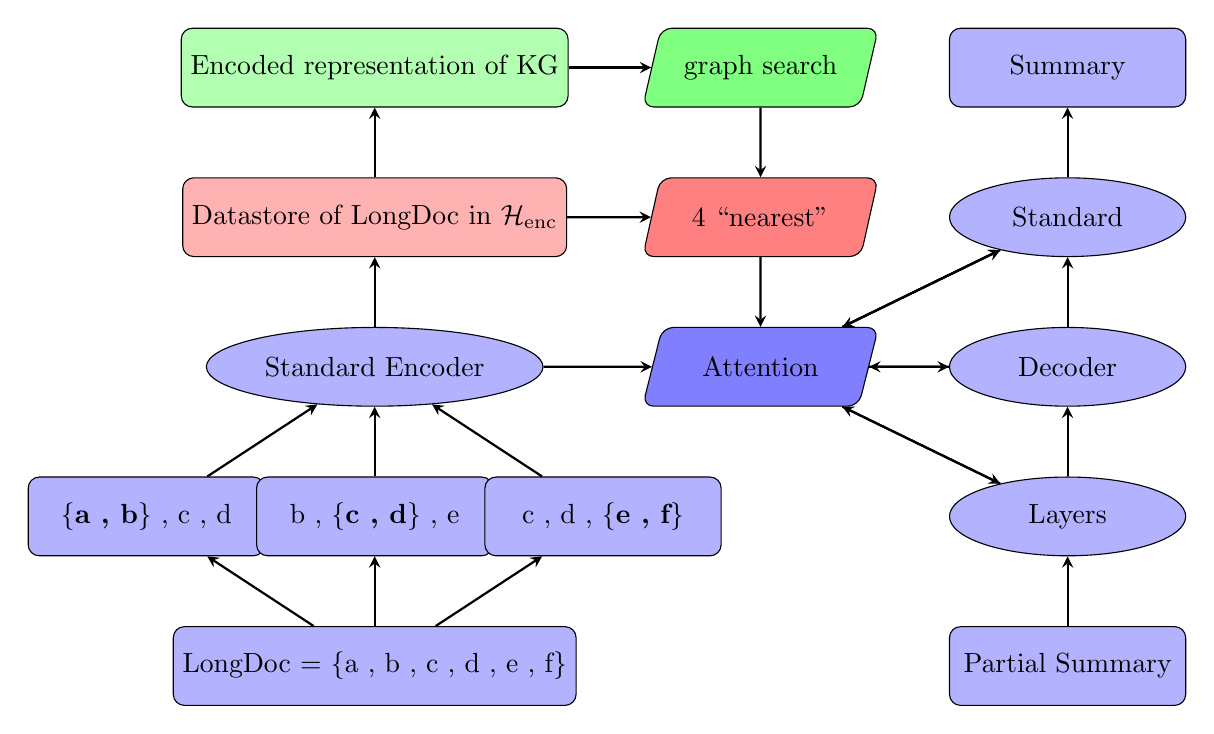
\begin{tikzpicture}[node distance=1.9cm]

%-----------chunks
  \node (chunk1) [startstop] {\{{\bf a , b}\} , c , d};
  \node (chunk2) [startstop, right of=chunk1, xshift=1cm] {b , \{{\bf c , d}\} , e};
  \node (chunk3) [startstop, right of=chunk2, xshift=1cm] 
    {c , d , \{{\bf e , f}\}};
%-----------the long document
\node[draw, rectangle, minimum width=4cm, minimum height=1cm,
  below of=chunk2]
  (longdoc) [startstop]{LongDoc = \{a , b , c , d , e , f\}};
%-----------the encoder
\node (encoder)[decision, above of=chunk2, xshift=0cm] {Standard Encoder};

%-----------the attention mechanism
\node (attn) [standardFn, right of=encoder, xshift=3cm] {Attention};

%-----------unlimiformer-----------
%-----------the datastore
\node[draw, rectangle, fill=red!30, minimum width=4cm, minimum height=1cm,
  above of=encoder, xshift=0cm, rounded corners]
  (datastore) {Datastore of LongDoc in $\mathcal H_\text{enc}$};
%-----------selecting the k nearest
\node (nearest) [unlimiFn, above of=attn] {$4$ ``nearest''};

%-----------combined model
\node[draw, rectangle, fill=green!30, minimum width=4cm, minimum height=1cm,
  above of=datastore, rounded corners]
  (kg) {Encoded representation of KG
%    $2^{\mathcal H_\text{enc}} \times 2^{\mathcal H_\text{enc}}$
  };
%-----------the alternative search
\node (search) [combFn, above of=nearest] {graph search};
%

%-----------decoder
\node (decoder2) [decision, right of=attn, xshift=2cm, yshift=0cm]
  {Decoder};
%-----------decoder
\node (decoder1) [decision, below of=decoder2]
  {Layers};
%-----------decoder
\node (decoder3) [decision, above of=decoder2]
  {Standard};

%-----------partial summary
\node (parsum) [startstop, below of=decoder1] {Partial Summary};
%-----------final summary
\node (sum) [startstop, above of=decoder3] {Summary};

\draw [arrow] (longdoc) -- (chunk1);
\draw [arrow] (longdoc) -- (chunk2);
\draw [arrow] (longdoc) -- (chunk3);
\draw [arrow] (chunk1) -- (encoder);
\draw [arrow] (chunk2) -- (encoder);
\draw [arrow] (chunk3) -- (encoder);
\draw [arrow] (encoder) -- (datastore);
\draw [arrow] (datastore) -- (kg);
\draw [arrow] (datastore) -- (nearest);
\draw [arrow] (kg) -- (search);
\draw [arrow] (search) -- (nearest);
\draw [arrow] (nearest) -- (attn);
\draw [arrow] (decoder1) -- (attn);
\draw [arrow] (decoder2) -- (attn);
\draw [arrow] (decoder3) -- (attn);
\draw [arrow] (attn) -- (decoder3);
\draw [arrow] (attn) -- (decoder1);
\draw [arrow] (attn) -- (decoder2);
\draw [arrow] (attn) -- (decoder3);
\draw [arrow] (encoder) -- (attn);
\draw [arrow] (parsum) -- (decoder1);
\draw [arrow] (decoder1) -- (decoder2);
\draw [arrow] (decoder2) -- (decoder3);
\draw [arrow] (decoder3) -- (sum);

\end{tikzpicture}
\caption{\footnotesize A stylised transformer with length-$4$ context window
  (in blue).  The standard approach to handling long documents is to process
  consecutive overlapping chunks of tokens sequentially. In red,
  \texttt{unlimiformer} augments this process by creating a complete datastore
  and selecting which tokens are fed into the attention mechanism. We augment this
process further using a Knowledge Graph to aid selection.} \label{fig-latex}
\end{figure}

%\begin{figure}[ht]
%  \centering \includegraphics[scale=0.27]{images/combinedmodel_2.png}
%  \caption{Building the KG via entity extraction and a slightly different
%  architecture}
%  \label{fig-extraction}
%\end{figure}

%
%\begin{tikzpicture}[node distance=1cm, auto, 
%    box/.style={draw, rectangle, minimum width=1cm, minimum height=0.8cm, align=center},
%    every path/.style={-latex, thick}]
%
%% Nodes
%\node[draw, rectangle, fill=gray!30, minimum width=4cm, minimum height=1cm] (input) {Index of one long input};
%\node[draw, rectangle, below=2cm of input] (encoder) {Encoder};
%\node[draw, rectangle, fill=green!30, right=2.5cm of encoder] (knn) {kNN Search};
%\node[draw, rectangle, fill=green!30, above right=0.5cm and 1cm of knn] (query) {query};
%\node[box, below=1cm of encoder] (a1) {a};
%\node[box, right=0.1cm of a1] (b1) {b};
%\node[box, right=0.1cm of b1] (c1) {c};
%\node[box, right=0.1cm of c1] (d1) {d};
%\node[box, right=0.1cm of d1] (e1) {e};
%\node[box, right=0.1cm of e1] (f1) {f};
%\node[box, below=1cm of a1] (a2) {a};
%\node[box, right=0.1cm of a2] (b2) {b};
%\node[box, right=0.1cm of b2] (c2) {c};
%\node[box, right=0.1cm of c2] (d2) {d};
%\node[box, right=0.1cm of d2] (e2) {e};
%\node[box, right=0.1cm of e2] (f2) {f};
%
%% Connectors
%\draw[thick] (input.south) -- (encoder.north);
%\draw[thick] (encoder.east) -- (knn.west);
%\draw[thick] (knn.north) |- (query.east);
%\draw[thick] (query.west) -| (c1.north);
%\draw[dashed, thick] (query.south) -| (c2.north);
%
%\end{tikzpicture}
%\begin{tikzpicture}[node distance=1cm, auto]
%
%% Nodes
%\node[draw, rectangle, fill=gray!30, minimum width=4cm, minimum height=1cm] (input) {Index of one long input};
%\node[draw, rectangle, below=of input, minimum width=2cm, minimum height=1cm] (encoder) {Encoder};
%\node[draw, rectangle, right=2cm of encoder, fill=green!30, minimum width=2cm, minimum height=1cm] (knn) {kNN Search};
%\node[draw, rectangle, right=2cm of knn, minimum width=2cm, minimum height=1cm] (decoder) {Decoder Layer};
%\node[draw, rectangle, below=of decoder, fill=blue!30, minimum width=2cm, minimum height=1cm] (cross) {Cross attention};
%\node[draw, rectangle, below=2cm of knn, fill=green!30, minimum width=1cm, minimum height=0.8cm] (query) {query};
%
%% etc... you would continue to define the rest of the nodes similarly
%
%% Connectors
%\draw[-{Triangle[width=3mm,length=3mm]}, thick] (input) -- (encoder);
%\draw[-{Triangle[width=3mm,length=3mm]}, thick] (encoder) -- (knn);
%% etc... you would continue to define the rest of the arrows similarly
%
%\end{tikzpicture}
%
%\begin{tikzpicture}[node distance=1cm, auto,
%    box/.style={draw, rectangle, minimum width=1cm, minimum height=0.8cm},
%    bigbox/.style={draw, rectangle, minimum width=3cm, minimum height=1.5cm},
%    every path/.style={-latex, thick}]
%
%% Nodes
%\node[draw, rectangle, fill=gray!30, minimum width=4cm, minimum height=1cm]
%  (input) {Index of one long input};
%\node[bigbox, below=1.5cm of input] (encoder) {Encoder};
%\node[bigbox, right=2cm of encoder, fill=green!30] (knn) {kNN Search};
%\node[bigbox, right=2cm of knn] (decoder) {Decoder Layer};
%\node[draw, rectangle, below=1.5cm of decoder, fill=blue!30, minimum width=2cm, minimum height=1cm] (cross) {Cross attention};
%\node[box, below=0.5cm of knn, fill=green!30] (query) {query};
%\node[box, left=0.5cm of query] (state) {Retrieved hidden states};
%\node[box, below=3cm of encoder, yshift=0.5cm] (a1) {a};
%\node[box, right=0.1cm of a1] (b1) {b};
%\node[box, right=0.1cm of b1] (c1) {c};
%\node[box, right=0.1cm of c1] (d1) {d};
%\node[box, right=0.1cm of d1] (e1) {e};
%\node[box, right=0.1cm of e1] (f1) {f};
%
%% Connectors
%\draw[thick]  (encoder.north) -- ++(0,0.5cm) -| (input.south);
%\draw[thick] (encoder) -- (knn);
%\draw[thick] (knn) -- (decoder);
%\draw[thick] (decoder.south) -- ++(0,-0.5cm) -| (cross.north);
%\draw[thick] (knn.south) -- (query);
%\draw[thick, dashed] (query) -- (state);
%\draw[thick, dashed] (query) -- (c1);
%
%% Add more connectors and nodes as requigray
%
%\end{tikzpicture}

\newpage
\end{document}
